%
% Introduction slides
%
\documentclass[compress,trans]{beamer}
%\documentclass{beamer}

\usepackage{graphicx}

\mode<presentation>
{
 \usetheme{default}
%%   \usetheme{Singapore}
  \setbeamertemplate{frametitle}[default][left]
  \setbeamercovered{transparent}
}

\usepackage[english]{babel}
% or whatever

\usepackage[latin1]{inputenc}
% or whatever

\usepackage{times}
\usepackage[T1]{fontenc}

\title{Nabu: A Data Publishing System Using ReST}
\subtitle{Python Training Presentation Slides}

\author{Martin Blais}

\institute{Furius Enterprise}

\date{February 2006}

\subject{Nabu Presentation @ PyCon 2006}

\setcounter{tocdepth}{4}

\newcommand{\todo}[1]{}


\AtBeginSubsection[]
{
  \begin{frame}<beamer>
    \frametitle{Outline}
    \tableofcontents[currentsection,currentsubsection]
  \end{frame}
}


% If you wish to uncover everything in a step-wise fashion, uncomment
% the following command: 
%\beamerdefaultoverlayspecification{<+->}

\begin{document}

%-------------------------------------------------------------------------------
\begin{frame}
  \titlepage
\end{frame}

%-------------------------------------------------------------------------------
\begin{frame}
  \frametitle{Outline}
  \tableofcontents
  % You might wish to add the option [pausesections]
\end{frame}

%===============================================================================



% \begin{frame}
%   \frametitle{Intro - Desktop Search}
% 
% So you have Google Desktop indexing your personal data on your computer\dots
% wouldn't it be great if this indexing database could be used to feed
% some of your blog automatically?
% 
% Wouldn't it be awesome if your personal address book would be formed
% automatically by having a system find all the addresses in all of your
% documents?
% 
% In this talk I will show a simple system that leverages docutils to do
% something like that.
% 

% - Try out Emacs Planner from Sasha, try it, see if I can get some ideas for
%   Nabu.


% %-------------------------------------------------------------------------------
% \begin{frame}
%   \frametitle{Motivation}
% 
% slide with the problem to solve
% 
% 
% \end{frame}
% 
% 
% - I write lots of little text files
% 
%   ... example ...
% 
%   - Configuration notes
% 
%     -> as these notes
% 
%   - Timesheet
% 
% 
% 
% What is Nabu?
% =============
% 
% - show diagram
% 
% 
% 
% 
% Example Extractor
% =================
% 
% - go through an example of writing an extractor
% 
% 
% 
% 
% 
% Applications
% ============
% 
% - blog
% 
%   - selective delivery of information
% 
%     e.g. ``soft privileges'', a link that expires, that allows access to a
%     specific resource, e.g. I want to share my image gallery with my boss
% 
% - calendar
% - timesheet
% 
% - ...
% 
% 
% Advantages
% ==========
% 
% - Any document structures can be reused and combined to provide a rich content
% 
% 
% 
% Downsides
% =========
% 
% - You have to understand how restructuredtext gets parsed
% 
%   - You end up getting dragged into the docutils project a bit
% 
%   --> You can use rst2pseudoxml.py to easily debug and learn input syntaxes
% 
% 
% Future Work
% ===========
% 
% - Support encryption in the publisher
% - Support per-document options (... adds complexity)
% 
% 



% 
% ========================================================
%   Strike Two -- Ideas for the talk from Rachel's place
% ========================================================

%-------------------------------------------------------------------------------
\begin{frame}[fragile]
  \frametitle{Introduction}

  I'm going to take a long winding road to introduce this project via a set of
  PIM examples\dots

\vfill\pause

  This will be an ode to the power and elegance of simple text files \dots


\end{frame}




%-------------------------------------------------------------------------------
\begin{frame}[fragile]
  \frametitle{1992 - Bookmarks}

  \begin{itemize}
    \item Xmosaic bookmarks
    \item Bookmarking lots of sites left and right
  \end{itemize}

\pause
A script was born (\verb@bmmgr@), typical input:


\begin{verbatim}
  Raymond Hettinger's photography
  http://www.knowyourboston.com
  photography, boston, sexy girls
\end{verbatim}

  \begin{itemize}
    \item Output to Xmosaic, then Netscape, then Mozilla, then IE \dots
    \item Eventually Firefox
    \item ... and what next?
  \end{itemize}

% - In 1992, I was using Xmosaic, the good old days of Linux had not arrived yet
% - Then Netscape came about, introduced some changes, and then Mozilla
% - I wanted to keep my preciously organized bookmarks from one browser to the next
% - In those days, bookmarks had more value, we did not have Google to help us out
% - At some point I had to use Windows, with yet another bookmarks format
% - Now I'm using Firefox, and I really don't know what I'll be using next
% - I wrote a small program to manage them, it would self-organize
% - This is a pattern in my life, solving little problems with scripts

\end{frame}

%-------------------------------------------------------------------------------
\begin{frame}[fragile]
  \frametitle{Bookmarks - Problems}

  A tree is inadequate, and organizing by hand is an annoyance

  \begin{itemize}
    \item Bookmarks belong in many nodes
    \item Sharing \textit{some} of these bookmarks (e.g. del.icio.us)
    \item Searching the bookmarks (too many bookmarks!)
  \end{itemize}

% - I wrote tengis, which is a small, simple database of bookmarks

\end{frame}


%-------------------------------------------------------------------------------
\begin{frame}[fragile]
  \frametitle{1997 - Address Book}

  \begin{itemize}
    \item Little paper booklets\dots

\vfill\pause

    \item Using Netscape to store my contacts in LDIF

\vfill\pause

    \item My MSc director, a nroff user, shows me his ascii system
  \end{itemize}

\vfill\pause

  \dots I've been living happily with text files since then \dots
  \begin{itemize}
    \item Using paragraph grep from a shell (e.g. \verb@pargrep.pl@)
  \end{itemize}

\vfill\pause

  \hfill \dots Or have I? 

\end{frame}


%-------------------------------------------------------------------------------
\begin{frame}[fragile]
  \frametitle{1999 - Blog}

  Before blogs were blogs\dots

  \begin{itemize}
  \item 199?: Phil Greenspun - \verb@photo.net@
  \item 1997: Patrick Jennings/Synaptic - cycling through China
  \item \dots I'm inspired: I write \dots another Python script.
  \end{itemize}

\vfill\pause

  \verb@adventures@ is born
  \begin{itemize}
    \item Grows into a monster
    \item Inputing XML was awful
    \item So I converted to input in ReStructuredText
    \item Regenerating static pages is not fun
  \end{itemize}

\end{frame}



% 200?
% ====
% 
% - I discover restructured text
% 
% FIXME: todo, check the age of docutils, when was it started?


%-------------------------------------------------------------------------------
\begin{frame}[fragile]
  \frametitle{2004 - The Art of Taking Notes}

  I'm getting a little bit old, losing memory\dots  \pause or maybe \\

\vfill

  I'm a little less stupid now and I just \textbf{KNOW} that I will forget. \\

\vfill\pause

  New task: I start a new text file to take notes.

  This is great, because:
  \begin{itemize}
    \item I can grep the files

    \item I can more easily interrupt my work

    \item Contains URLs in context, rather than in a global list

  \end{itemize}

  I would like to share many of these short technical documents when people
  ask questions \dots

\end{frame}


%-------------------------------------------------------------------------------
\begin{frame}[fragile]
  \frametitle{2005 - Travel Files - Mixed Data}

Travel notes:
\begin{itemize}
\item Things to do, personal notes, itineraries ($\rightarrow$ simple text)
\item Addresses of people to visit ($\rightarrow$ contact info)
\item URLs of related websites ($\rightarrow$ bookmarks)
\item References to books and articles ($\rightarrow$ publications)
\end{itemize}

%% \begin{verbatim}

%% \end{verbatim}


% .. <diagram with files and information stored across them>
% 
% What if I could identify and extract the meaningful parts of information from
% those files and store it appropriately?
% 
% What could I build with this?
% 
% - You may have heard this idea before: the Semantic Web
% 
%   It would allow searching the "address book" of the entire internet!
%
% - If anyone has a stab at this today, it's google
% - I think it will get better, but it will never be perfect
% 
% - Many years in the making, will probably never happen in its ideal form


\end{frame}


%-------------------------------------------------------------------------------
\begin{frame}[fragile]
  \frametitle{Wikis Suck}

Why?

\begin{itemize}

\item Anything but the most trivial title looks horrible:

\begin{verbatim}
  BrazilTravelNotes
\end{verbatim}

\item The editor facilities in most of the browsers is lame
  \begin{itemize}
  \item Who has never lost a file being edited in a browser?
  \end{itemize}

% * Cool idea: link an emacs instance within Firefox.
% * Does not identify the meanings within the files either.

\end{itemize}

\end{frame}





%-------------------------------------------------------------------------------
\begin{frame}[fragile]
  \frametitle{The Goal}

  Build a system that can extract semantically meaningful informations in my set
  of personal info files and store them in a structured way (in database
  tables), so I can use this information later and serve in new, interesting
  ways.

\end{frame}



%-------------------------------------------------------------------------------
\begin{frame}[fragile]
  \frametitle{What Nabu is not\dots}

Not a Wiki



\end{frame}



%-------------------------------------------------------------------------------
\begin{frame}[fragile]
  \frametitle{Overview}

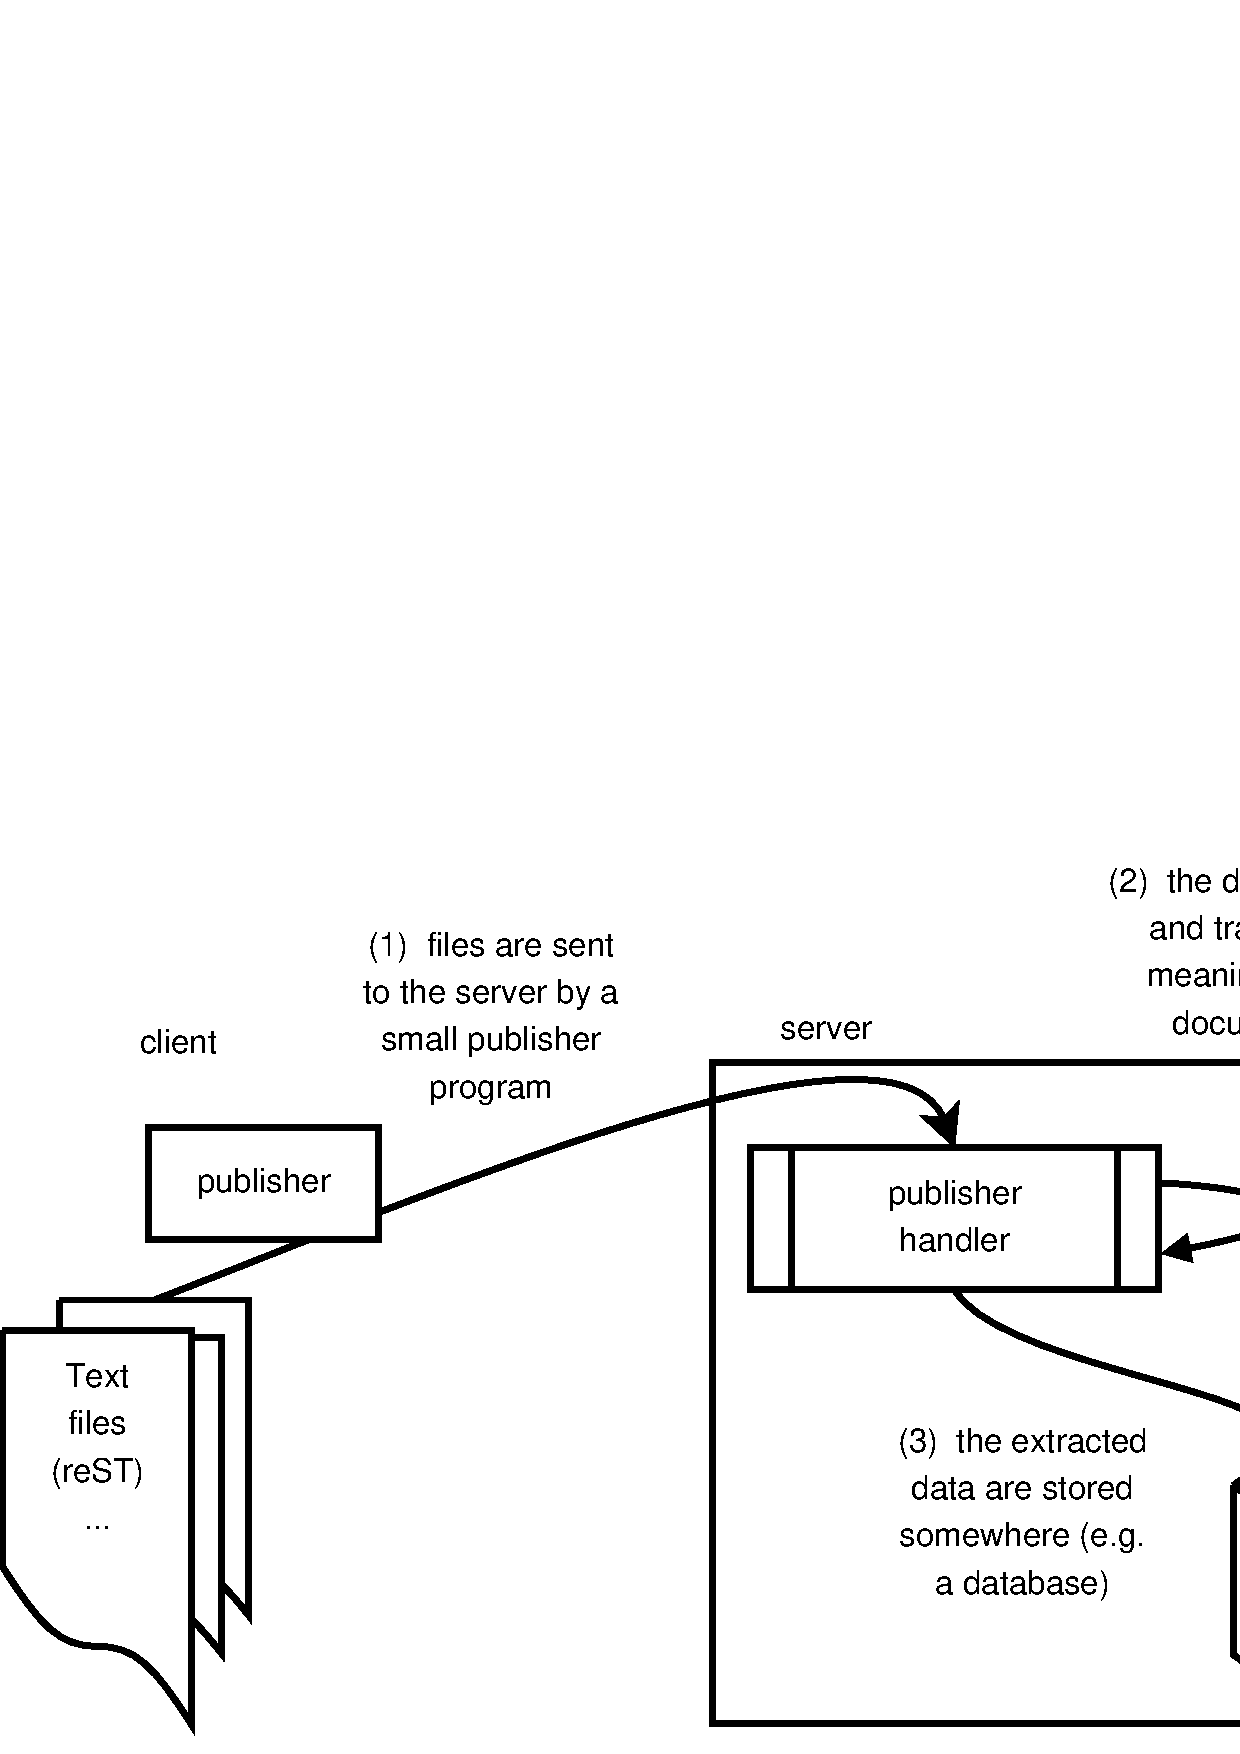
\includegraphics[width=1.0\textwidth]{../nabu2.pdf}

\end{frame}



%-------------------------------------------------------------------------------
\begin{frame}[fragile]
  \frametitle{Design}

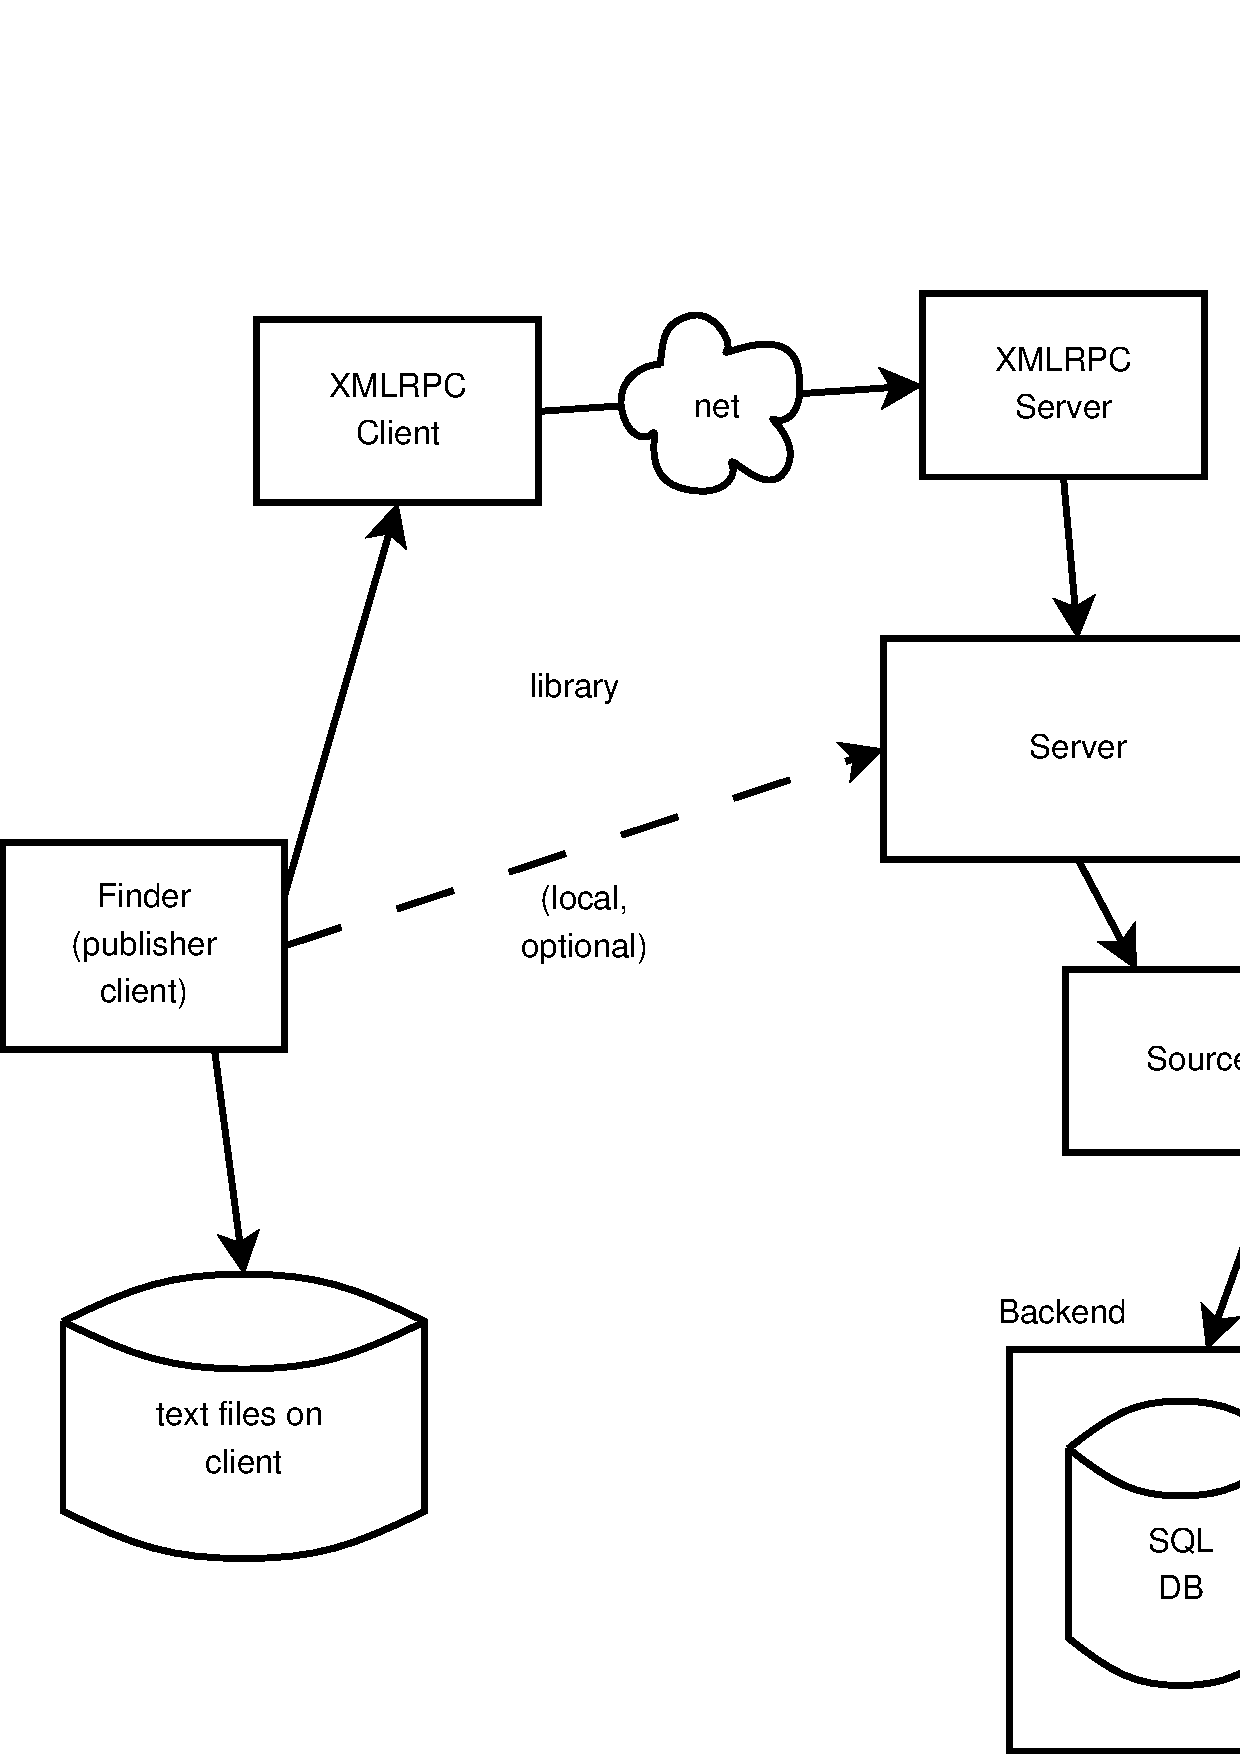
\includegraphics[width=1.0\textwidth]{../nabu1.pdf}

\end{frame}



%-------------------------------------------------------------------------------
\begin{frame}[fragile]
  \frametitle{Target Audience}
 
 Not for your mom!
\vfill
 
\pause
 Programmers have developed this great ability: to edit text files.
 
 \begin{itemize}
 \item we understand indentation
 \item we know spacing, justification, filling, etc.
 \end{itemize}
 
 Leverage it!
 
\end{frame}

 
%-------------------------------------------------------------------------------
\begin{frame}[fragile]
  \frametitle{Real Editing}

I live in Emacs.

When I first log in on my machine, I invariably do:
\begin{enumerate}
\item start a shell
\item start emacs
\item start a web browser
\end{enumerate}

Most of you are probably doing the same.

Emacs or vi are always kept running.
 
\end{frame}
 



% The Dependency Problem
% ======================
% 
% More dependencies means
% 
% - it's harder to install
% - it's usable on less platforms
% - the lifetime of the project is linked with the lifetime of the shorter
%   dependency
% 
% On the **client**, we depend only on:
% 
% - Python
% - Text files (i.e. files with one of the predefined encodings)
% 
% 
% 
% ReStructuredText
% ================
% 
% .. ask Goodger to get up
% 
%    "If you see this guy in the corridor, show him some love, give him a hug."
% 
% - The best text-to-structure conversion tool.
% - Finds the best compromises (all decisions are documented thoroughly)
% 
% 
% .. <show some text with recursive boxes in it>
% 
% 
% 
% 
% 
% Desktop Search
% ==============
% 
% Imagine if you could use your desktop database to feed your blog.













% FIXME: build a graph with the docutils structure, the one with
% reader/transform/writer, same as in the documentation, with the intention to
% explain that I've had to modify it and to stop the process halfway













%-------------------------------------------------------------------------------
\begin{frame}[fragile]
  \frametitle{Events Example}

\begin{verbatim}
sat 2005-12-31 19h30
  - NYE Evening chez Stuart

sat 2005-12-31 
  - Proteus: mkisofs for backup copy DVD-ROM

2006-01-02
  - Contact SonoMax about free earplugs
  - Track Leif's grille that was supposed to arrive.

2006-01-03
  - Visit Yves * D'ailleurs je vais avoir besoin de tes info pour les
    salaires de 2005

  - Confirm flight to Brazil w/ Constellation

2006-01-04 20h00 
  - Dinner w/ Pierre @ Golden Cari

2006-01-05
  - Book room for PyCon (should be 79 USD) in january when problems are fixed.

2006-01-13, 14, 16
  - Vote par anticipation

\end{verbatim}

\end{frame}


%-------------------------------------------------------------------------------
\begin{frame}[fragile]
  \frametitle{Calendar View}

\includegraphics[width=1.0\textwidth]{calendar-shot.pdf}

% Add this: I have dated events in my file for Brazil, PyCon, my TODO file, they
% all merge into my calendar.

\end{frame}



%-------------------------------------------------------------------------------
\begin{frame}[fragile]
  \frametitle{Nabu Contents Browser - Extracted}

\includegraphics[width=1.0\textwidth]{ll-extracted.pdf}

\end{frame}


%-------------------------------------------------------------------------------
\begin{frame}[fragile]
  \frametitle{Nabu Contents Browser - Upload Info}

\includegraphics[width=1.0\textwidth]{ll-upload.pdf}

\end{frame}





%-------------------------------------------------------------------------------
\begin{frame}[fragile]
  \frametitle{Problems}

- Creating precise reStructuredText can be fragile from the user's point-of-view

(EXAMPLE)

\end{frame}



%-------------------------------------------------------------------------------
\begin{frame}[fragile]
  \frametitle{Possible Uses}

... static site, with a small dynamic section

allows you to avoid having to write input forms

% - uses: imagine a static pages site, but you want to update the special events
%   yourself (the client pays for this).  You can do that with a simple text file
%   and Nabu.
% 



\end{frame}




%===============================================================================
\end{document}


% Add: MapExtractor that can extract all my links to Google maps and create a
% single map with them, or a list of locations, they could be accompanied with a
% trail, and then each trail be displayed separately

